\documentclass[a4paper,11pt]{article}
\usepackage[T1]{fontenc}
\usepackage[utf8]{inputenc}
\usepackage{lmodern}
\usepackage{graphicx}
\usepackage{subcaption}

\title{Reinforcement Learning results analysis}
\author{Marco Marini}

\begin{document}

\maketitle
\tableofcontents

\begin{abstract}
Reinforcement Learning results analysis.
\end{abstract}

\section{Measures}

One hundred tests were run a maze environment with two different hyper parameters configurations.

Each test consist of 1000 episodes with a limit of 300 steps per episode.

\begin{figure}[h!]
	\centering
	\begin{subfigure}[b]{0.4\linewidth}
		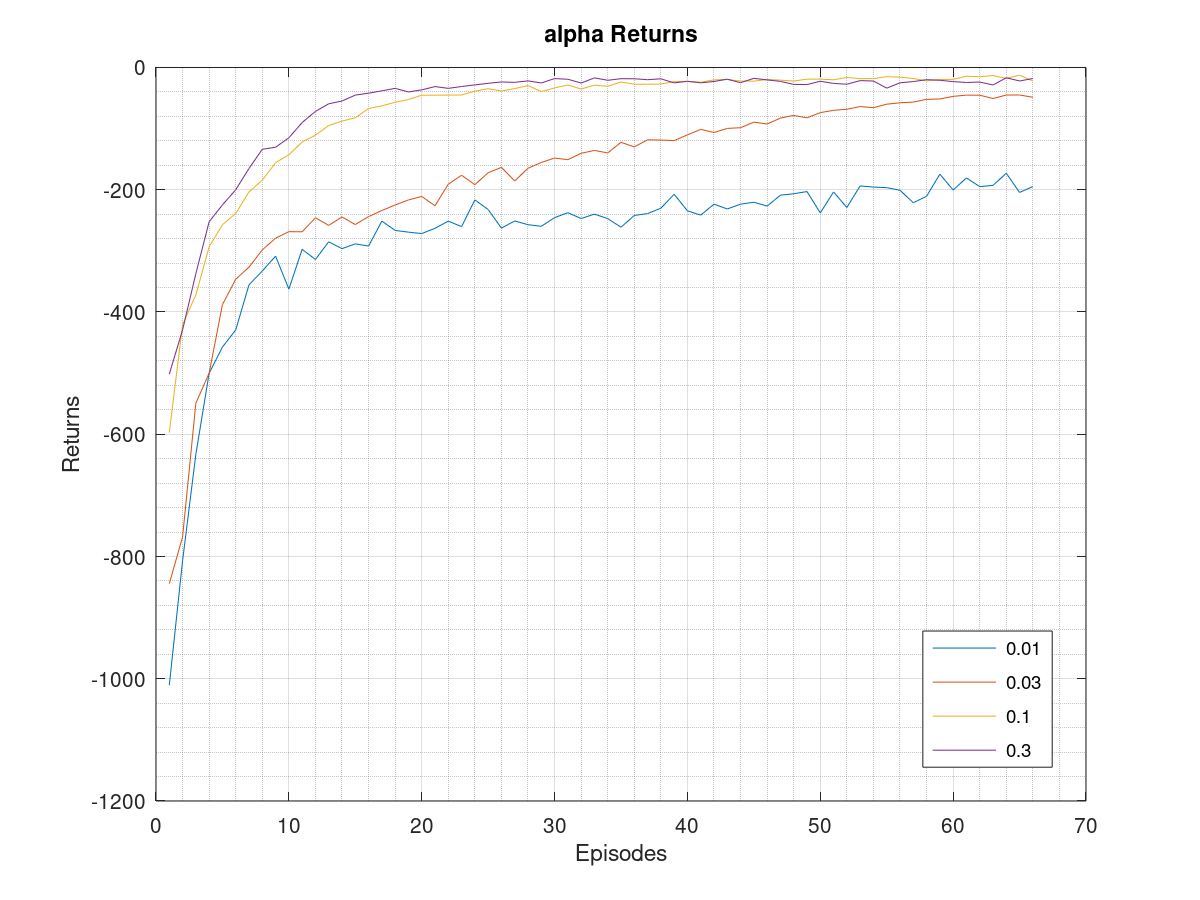
\includegraphics[width=\linewidth]{alpha-returns.png}
		\caption{$\alpha$ Returns.}
	\end{subfigure}
	\begin{subfigure}[b]{0.4\linewidth}
		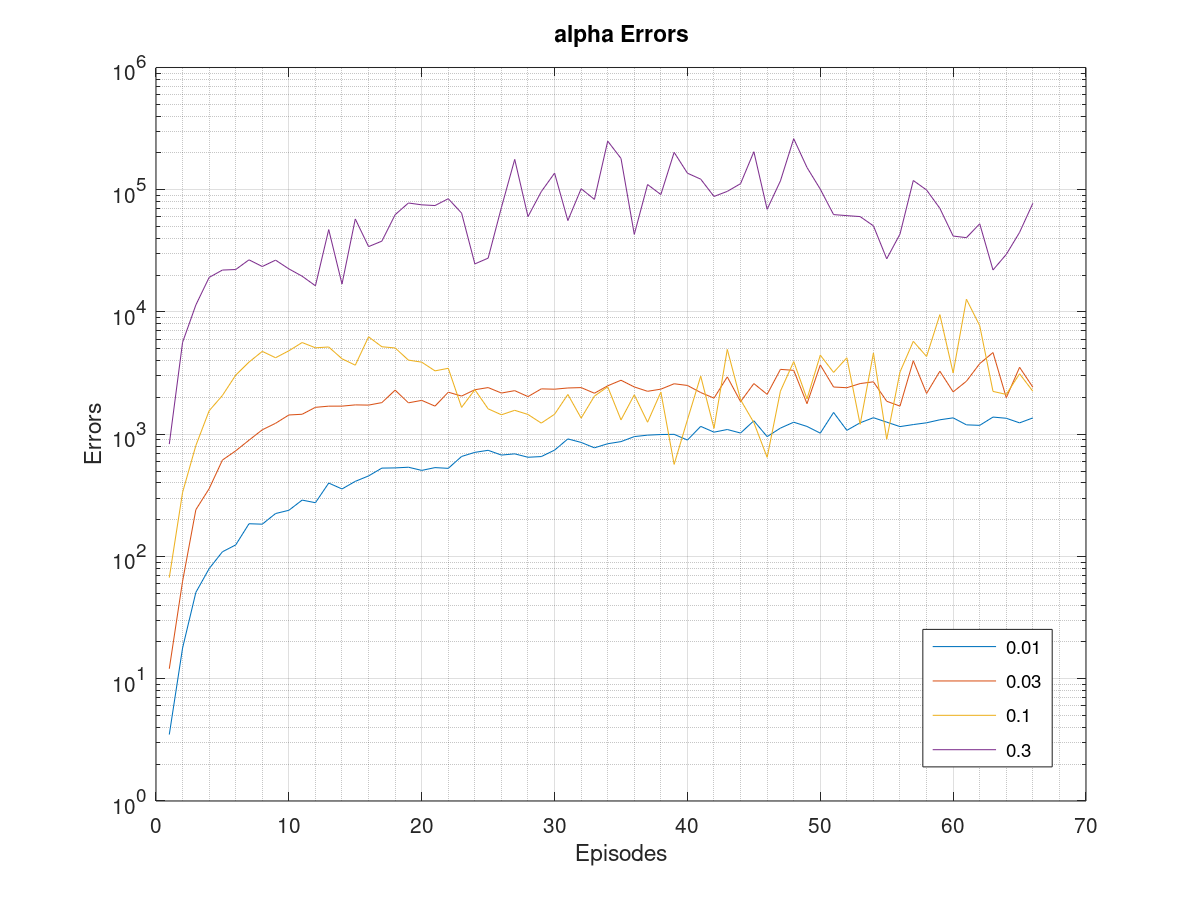
\includegraphics[width=\linewidth]{alpha-errors.png}
		\caption{$\alpha$ Errors.}
	\end{subfigure}

	\begin{subfigure}[b]{0.4\linewidth}
		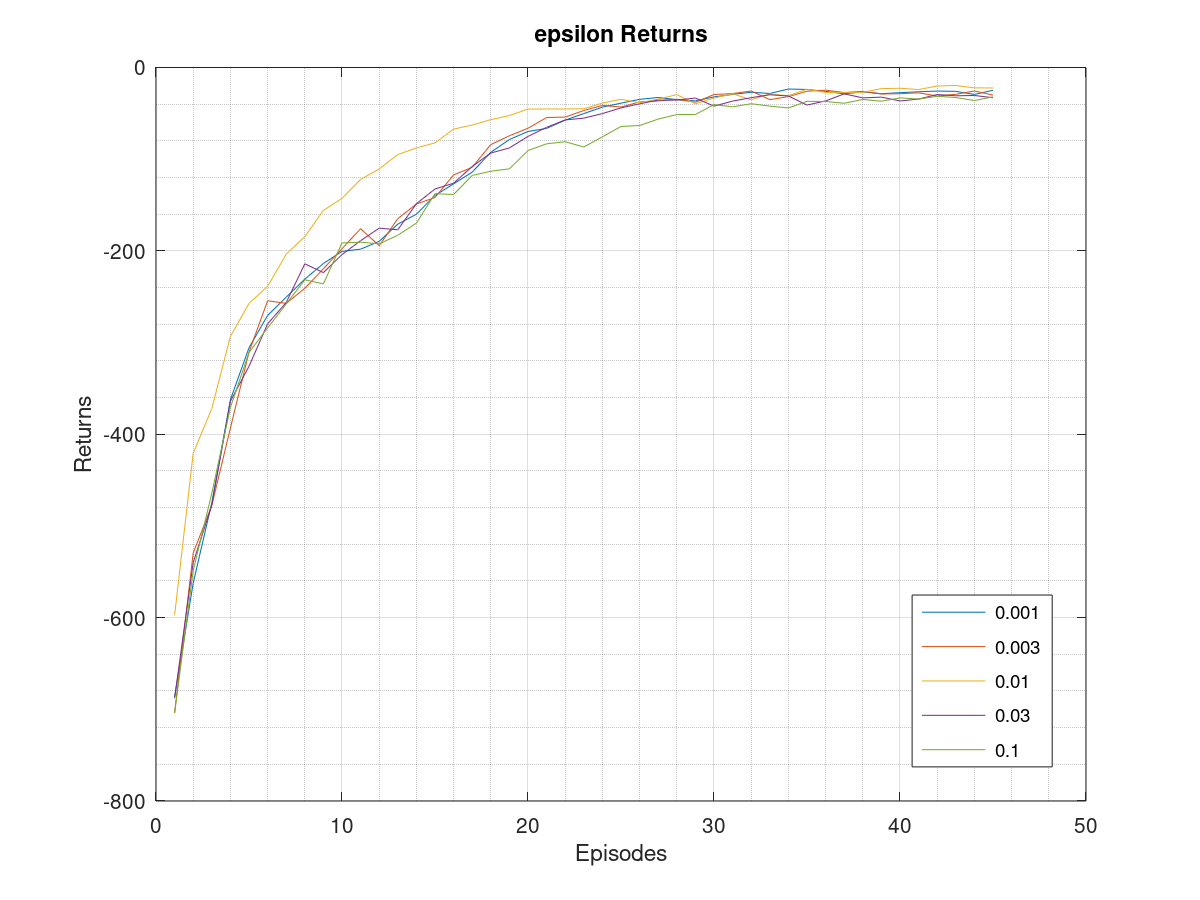
\includegraphics[width=\linewidth]{epsilon-returns.png}
		\caption{$\varepsilon$ Returns.}
	\end{subfigure}
	\begin{subfigure}[b]{0.4\linewidth}
		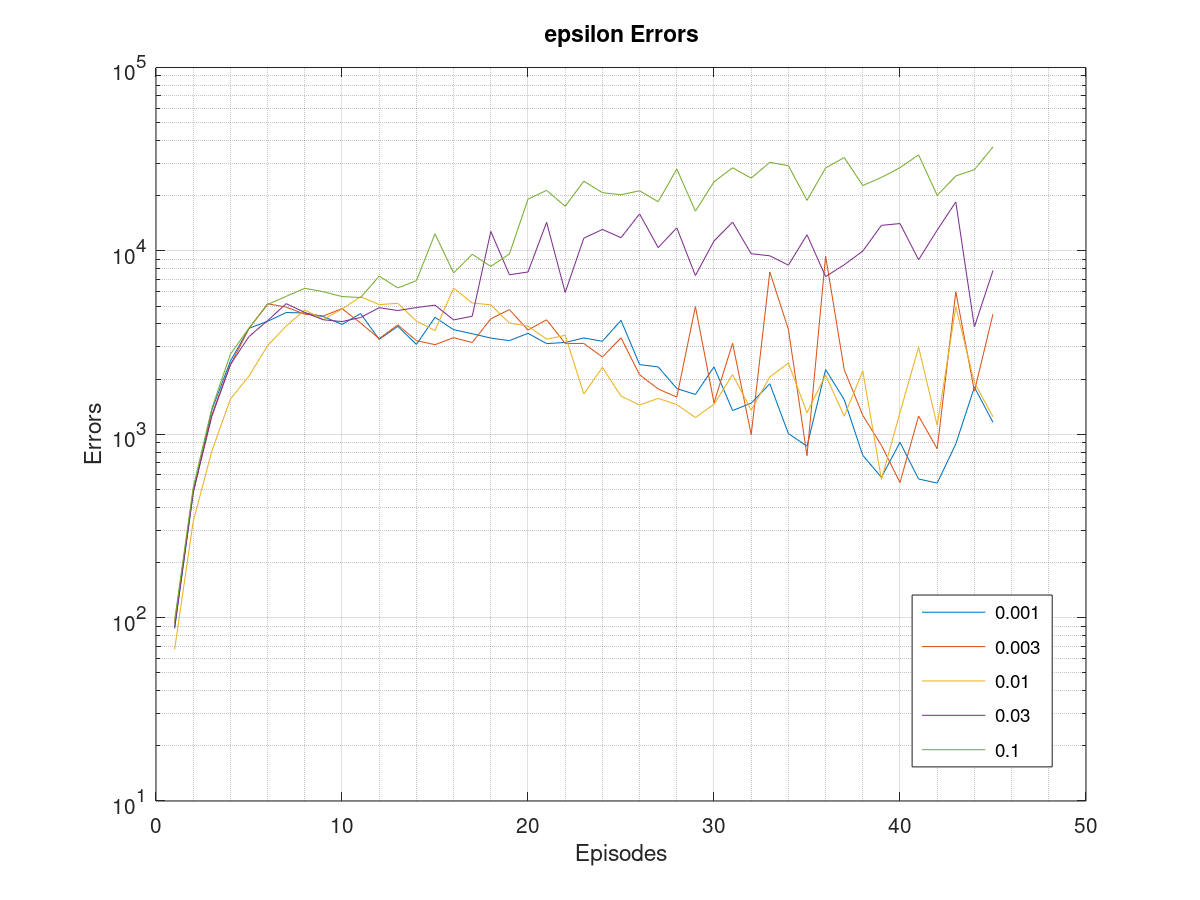
\includegraphics[width=\linewidth]{epsilon-errors.png}
		\caption{$\varepsilon$ Errors.}
	\end{subfigure}

	\begin{subfigure}[b]{0.4\linewidth}
		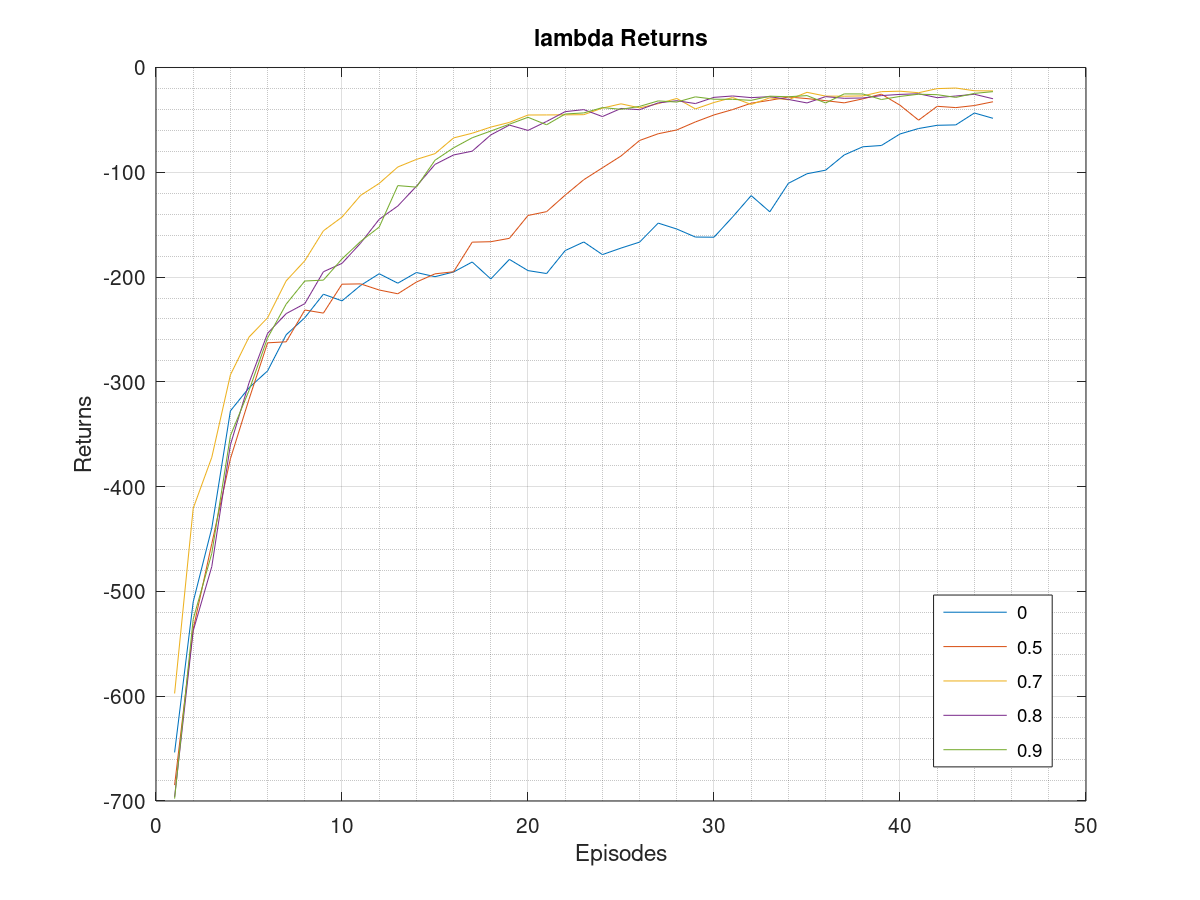
\includegraphics[width=\linewidth]{lambda-returns.png}
		\caption{$\lambda$ Returns.}
	\end{subfigure}
	\begin{subfigure}[b]{0.4\linewidth}
		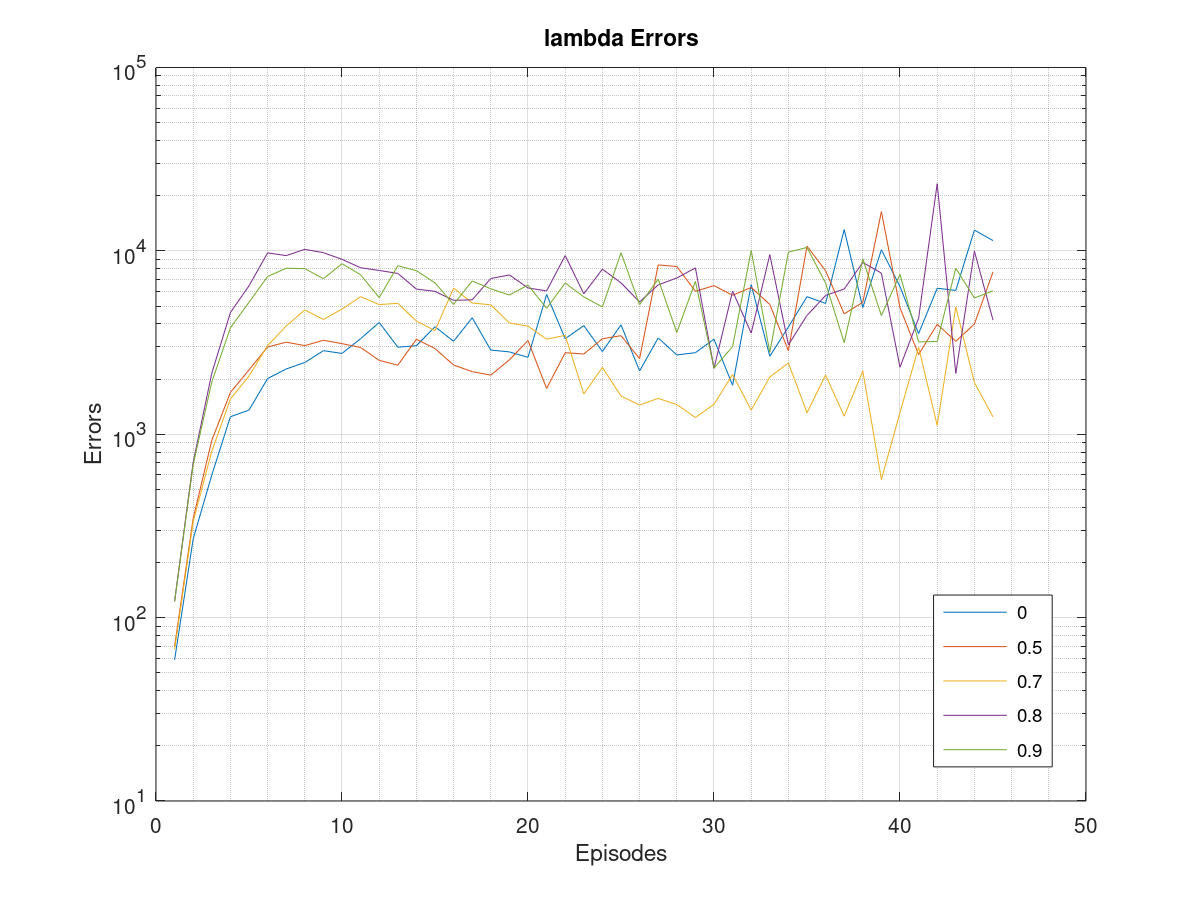
\includegraphics[width=\linewidth]{lambda-errors.png}
		\caption{$\lambda$ Errors.}
	\end{subfigure}

	\begin{subfigure}[b]{0.4\linewidth}
		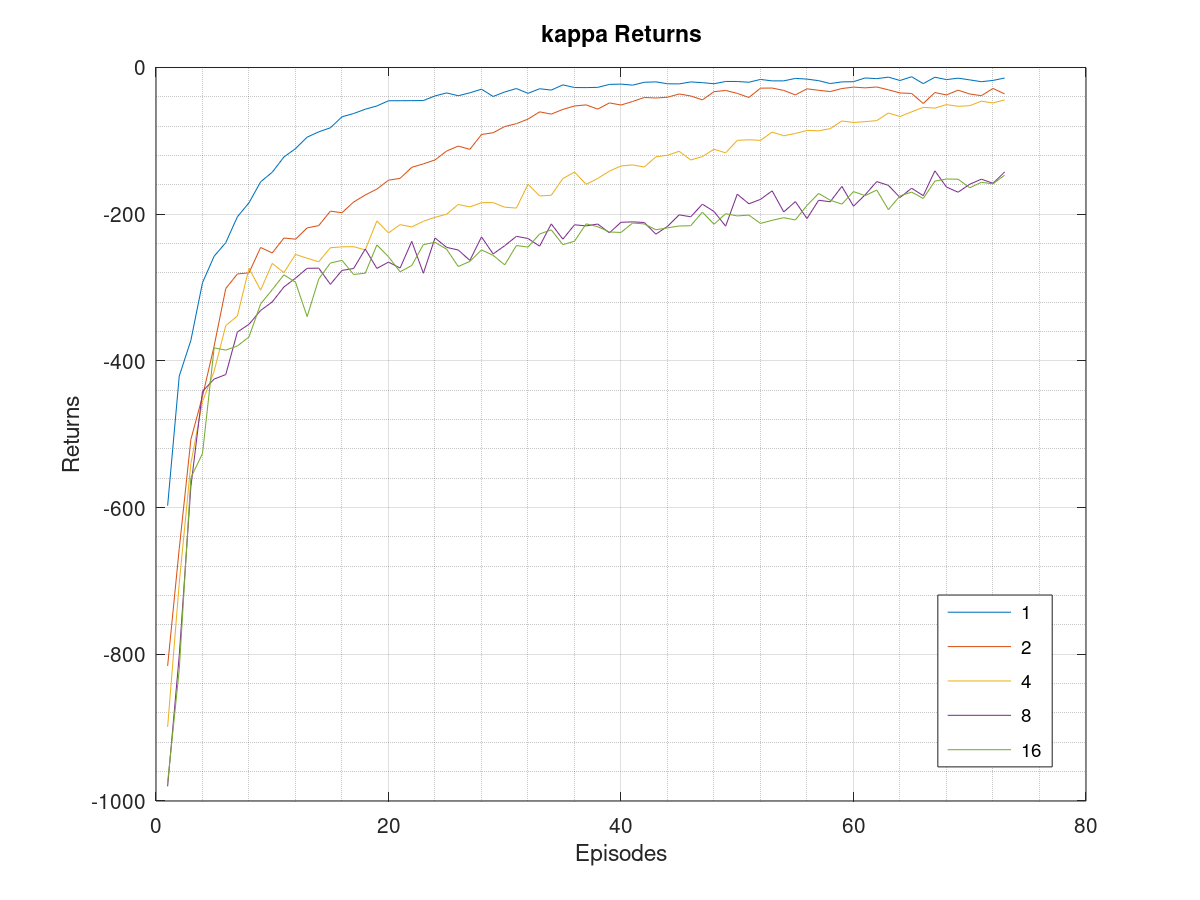
\includegraphics[width=\linewidth]{kappa-returns.png}
		\caption{$\kappa$ Returns.}
	\end{subfigure}
	\begin{subfigure}[b]{0.4\linewidth}
		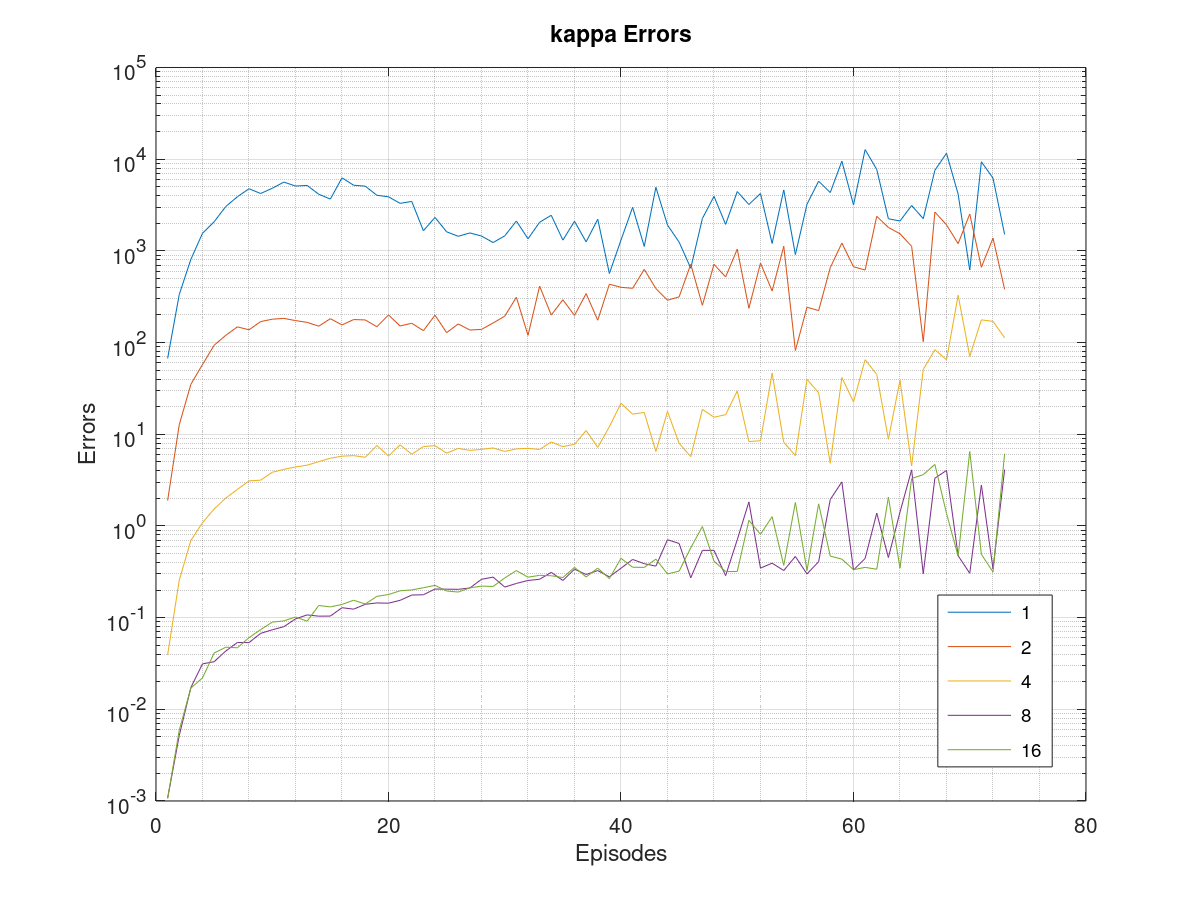
\includegraphics[width=\linewidth]{kappa-errors.png}
		\caption{$\kappa$ Errors.}
	\end{subfigure}

	\caption{Hyper parameters}
	\label{fig:hyper}
\end{figure}

\section{Adam optimizer}

The figure \ref{fig:adam} show the comparison between the SGD and ADAM alghoritm.

\begin{figure}[h!]
	\centering
	\begin{subfigure}[b]{0.4\linewidth}
		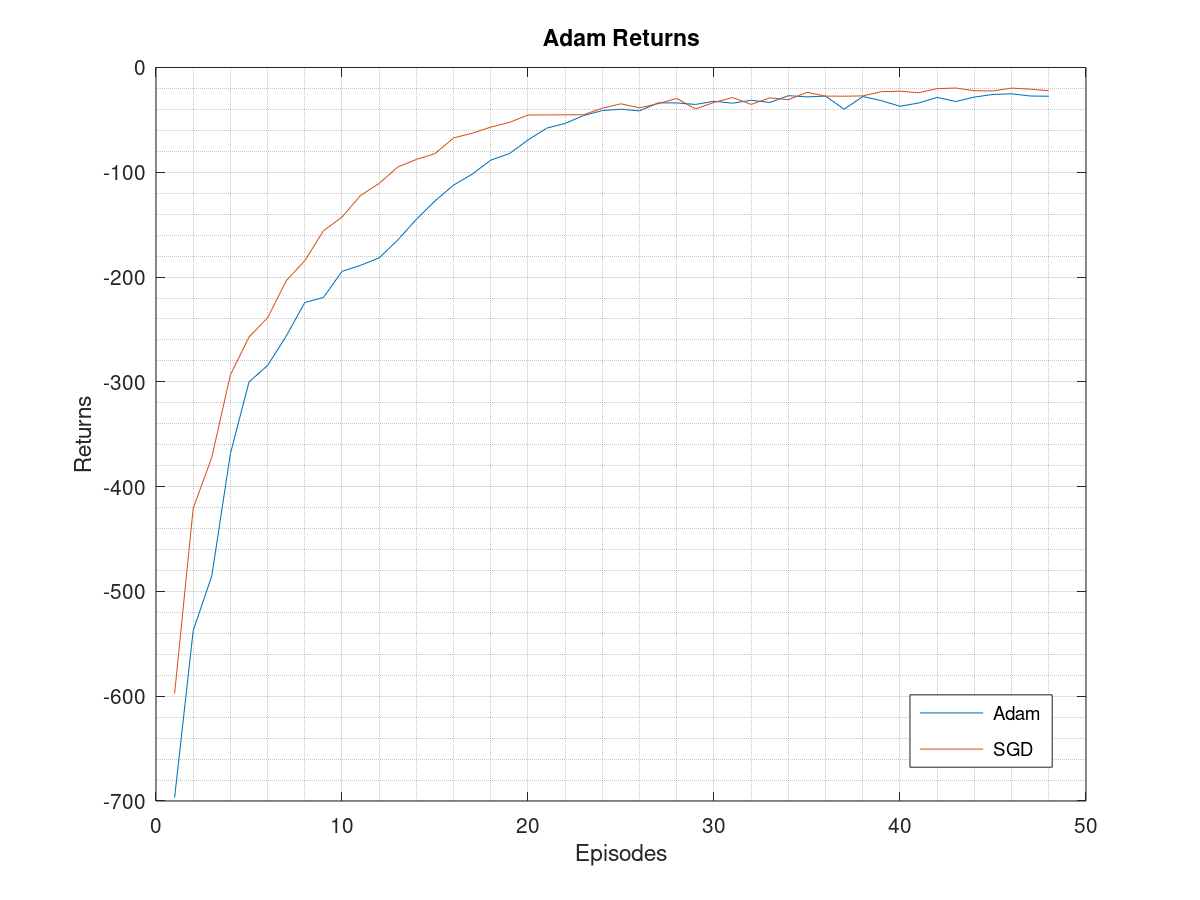
\includegraphics[width=\linewidth]{Adam-returns.png}
		\caption{$\alpha$ Returns.}
	\end{subfigure}
	\begin{subfigure}[b]{0.4\linewidth}
		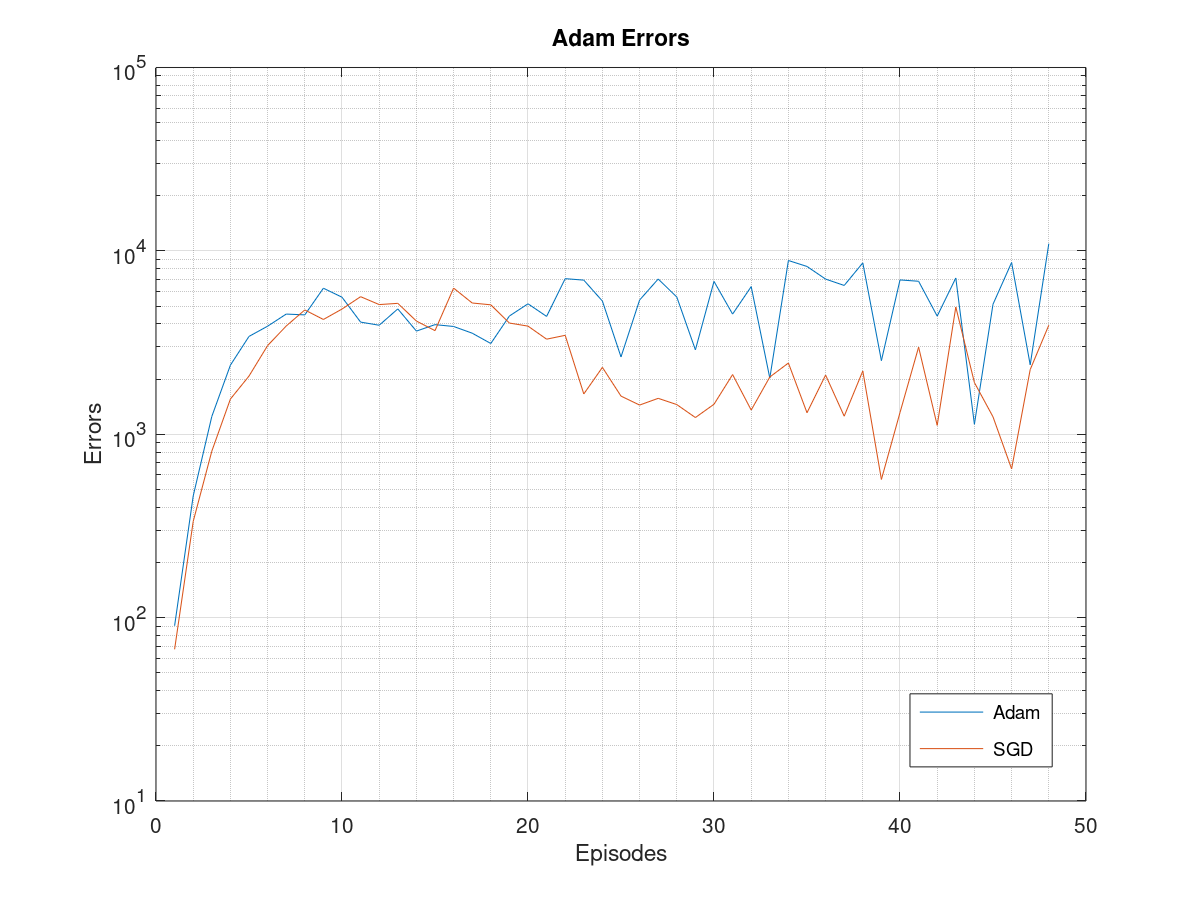
\includegraphics[width=\linewidth]{Adam-errors.png}
		\caption{$\alpha$ Errors.}
	\end{subfigure}
	
	\caption{Adam optimizer}
	\label{fig:adam}
\end{figure}

\end{document}